
%---------------------------------------------------------------------
%	PAKKER
%---------------------------------------------------------------------

\documentclass[12pt,fleqn,a4paper]{report}
\usepackage[utf8]{inputenc}
\usepackage[danish]{babel}
\usepackage[top=2.5cm, left=2cm, right=2cm, bottom=2.5cm]{geometry}
\usepackage{graphicx}
\usepackage[bottom]{footmisc}
\usepackage{framed}
\usepackage{caption}
\usepackage{mdframed}
\usepackage{listings}
\usepackage{color}
\usepackage[T1]{fontenc}
\usepackage{amsmath,amsfonts,amsthm} % Math packages
\usepackage{array}
\usepackage{wrapfig}
\usepackage{multirow}
\usepackage{tabu}
\usepackage{lastpage}
\usepackage{fancyhdr}
\usepackage[compact]{titlesec}
\usepackage[table,xcdraw]{xcolor}
\usepackage{arydshln}
\usepackage{mdframed}
\definecolor{mygreen}{RGB}{28,172,0} % color values Red, Green, Blue
\definecolor{mylilas}{RGB}{170,55,241}
\renewcommand{\lstlistingname}{Kodeudsnit}
\tabulinesep=3mm


\lstset{language=Matlab,%
    %basicstyle=\color{red},
    breaklines=true,%
    morekeywords={matlab2tikz},
    keywordstyle=\color{blue},%
    morekeywords=[2]{1}, keywordstyle=[2]{\color{black}},
    identifierstyle=\color{black},%
    stringstyle=\color{mylilas},
    commentstyle=\color{mygreen},%
    showstringspaces=false,%without this there will be a symbol in the places where there is a space
    emph=[1]{for,end,break},emphstyle=[1]\color{red}, %some words to emphasise
    %emph=[2]{word1,word2}, emphstyle=[2]{style},    
}


\makeatletter
\pagestyle{fancy}
\fancypagestyle{plain}{}
\fancyfoot{} % clear all fields
\fancyfoot[RO,RE]{Side \thepage\ af \pageref{LastPage}}
\fancyhead{} % clear all fields
\renewcommand{\headrulewidth}{0pt}

\def\thickhrulefill{\leavevmode \leaders \hrule height 1.2ex \hfill \kern \z@}
\def\@makechapterhead#1{
  \vspace*{10\p@}%
  {\parindent \z@ \centering \reset@font
        \thickhrulefill\quad 
        \scshape\bfseries\textit{\@chapapp{}  \thechapter}  
        \quad \thickhrulefill
        \par\nobreak
        \vspace*{10\p@}%
        \interlinepenalty\@M
        \hrule
        \vspace*{10\p@}%
        \Huge \bfseries #1 \par\nobreak
        \par
        \vspace*{10\p@}%
        \hrule
        \vskip 40\p@
  }}


\titlespacing{\subsection}{20pt}{*2}{*2}
\titlespacing{\subsubsection}{40pt}{*2}{*2}

\graphicspath{ {Figur/} }


%På figur~\ref{fig:fuld_lyd_tid}


%\begin{framed}
%\begin{center}
%	\includegraphics[width=\textwidth]{fuld_lyd_tid.png}
%	\captionof{figure}{Trafikstøj set i forhold til tiden} 
%	\label{fig:fuld_lyd_tid}
%\end{center}
%\end{framed}



%Se Kodeudsnit \ref{lstlisting:generel_kode}

%\captionof{lstlisting}{Generelle egenskaber for koden til fremstilling af diverse figure i matlab} 
%\label{lstlisting:generel_kode}
%\vspace{5mm} %5mm vertical space
%
%\subsection{Kode til lyd i forhold til tiden}
%\begin{framed}
%\begin{center}
%\begin{lstlisting}
%figure('name','trafikstoejen i fuld laengde'); clf
%subplot(211);
%plot(t,s_sound_left)
%xlabel('Tid (sek)')
%ylabel('Signalstyrke')
%title('Trafikstoej set i forhold til tiden')
%grid on
%hold on
%\end{lstlisting}
%\end{center}
%\end{framed}




\begin{document}
	
%---------------------------------------------------------------------
%	FORSIDE
%---------------------------------------------------------------------

\begingroup
\thispagestyle{empty}
\centering
\vspace*{5cm}
\par\normalfont\fontsize{35}{35}\sffamily\selectfont
\textbf{UDP socket fil overførsel}\\
{\LARGE IKN øvelse 8}\par
{\LARGE Gruppe 52}\par
\vspace*{1cm}
{\small
\begin{center}
\begin{tabu} to 1 \textwidth { X[l,1]  X[c,1] X[c,1] }
	Ragnar-Gwyn Dixen & 201400301 & au516263\\
	Thomas Sanberg Jensen & 201401914 & au513522\\
	Benjamin Kirkeby & 201410819 & au529001\\
	\end{tabu}
\end{center}}
\endgroup
\newpage


%---------------------------------------------------------------------
%	INDHOLD
%---------------------------------------------------------------------
\tableofcontents{}
\newpage

%---------------------------------------------------------------------
%	INDLEDNING
%---------------------------------------------------------------------
\chapter{Indledning}

\section{Opgaveformulering}
Denne journal skal beskrive udviklingsforløbet, funktionaliteten og resultatet for udviklingen af:
\begin{enumerate}
	\item Skriv en iterativ UDP-server med support for en client ad gangen, som kan modtage en forespørgsel fra en client.
	Forespørgslen fra client til server kan være en af to muligheder: ”U” eller ”L”. Om bogstaverne er lower case eller upper case skal være ligegyldigt.
	\begin{itemize}
		\item Hvis serveren modtager et ”U” skal informationen i filen /proc/uptime
		returneres til client. Denne fil indeholder aktuel information om den samlede
		tid serveren har været kørende siden opstart.
		\item Hvis serveren modtager et ”L” skal informationen i filen /proc/loadavg
		returneres til client. Denne fil indeholder aktuel information om serverens aktuelle CPU-load.
	\end{itemize}
	
	\item Skriv en UDP-client kørende i en anden laptop eller virtuel maskine, som kan sende en kommando i form af et bogstav ”U”, ”u”, ”L”, ”l” som indtastes af operatøren til UDP-serveren. Når svaret fra UDP-serveren (beskrevet i punkt 1) modtages, udskrives dette svar til UDP-client’s bruger. 
	
	\item Følgende figur (figur~\ref{fig:opstilling}) viser selve opstillingen, portnummer, brugerfladens syntax og , forslag til programmeringssprog:
	\begin{center}
		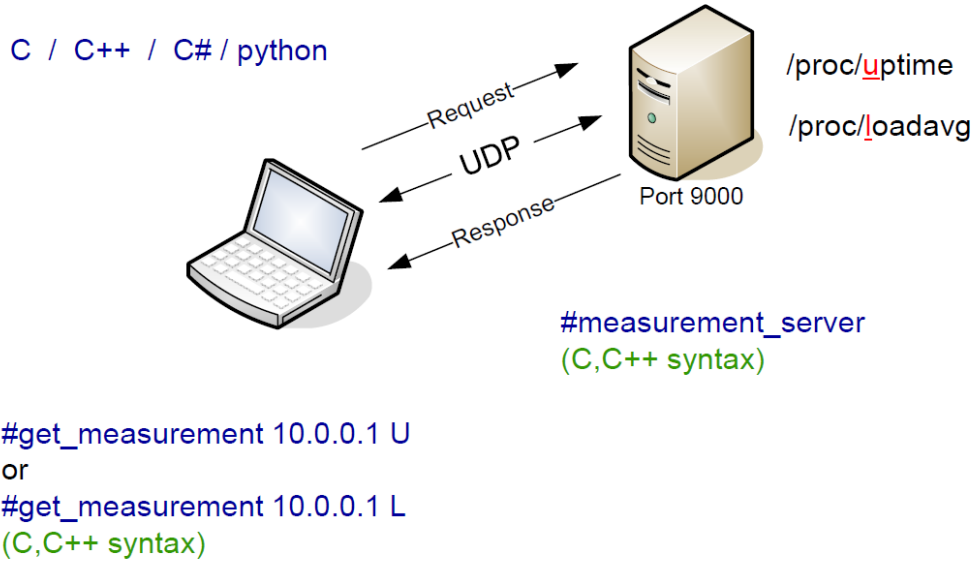
\includegraphics[width=0.7 \textwidth]{opstilling.png}
		\captionof{figure}{Opstilling af udp socket opstillingen}
		\label{fig:opstilling}
	\end{center}

\end{enumerate}

\chapter{Fremgangsmåde}
For at lave en udveksling mellem klient og server er der blevet gjort brug af følgende fremgangsmåde (figur~\ref{fig:opbygning}):
\begin{center}
	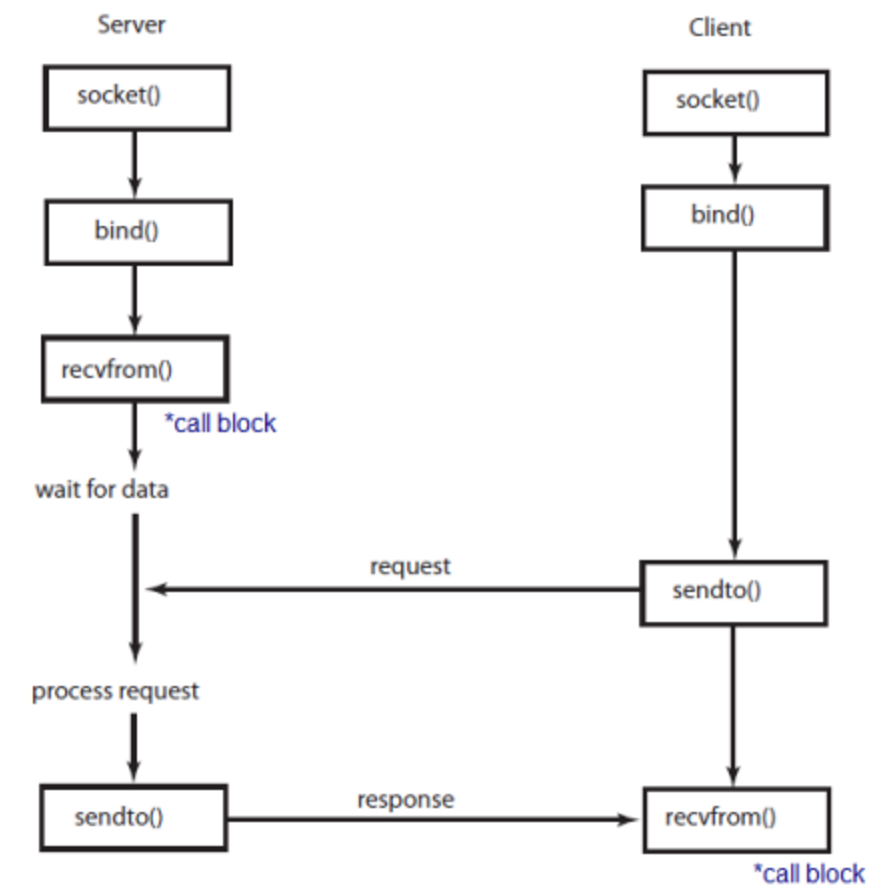
\includegraphics[width=0.7 \textwidth]{opbygning.png}
	\captionof{figure}{Opbygningen af UDP socket filudveksling}
	\label{fig:opbygning}
\end{center}

De enkelte blokke vil blive beskrevet i de følgende afsnit.

\newpage

\section{Socket() (Server \& Klient)}
I Kodeudsnit \ref{lstlisting:socket} ses hvordan socket bliver lavet. Denne kode er fælles for både server og klient.

\begin{framed}
	\begin{lstlisting}[language=C++]
//create a UDP socket
if ((socketfd=socket(AF_INET, SOCK_DGRAM, IPPROTO_UDP)) == -1)
{
	errormsg((char *)"socket");
}
\end{lstlisting}
\end{framed}
\captionof{lstlisting}{Socket bliver lavet} 
\label{lstlisting:socket}
\vspace{5mm} %5mm vertical space

\section{Bind() (Server \& Klient)}
Bind er forskelligt sat op på server siden og klient siden. Dette skyldes at serveren skal stå og lytte efter indkommende beskeder på porten, og er "ligeglad" med IP adressen, mens klienten skal vide hvilken server (altså IP-adresse) der ønskes forbindelse til. Derfor bliver portnummeret sat ind i socket på serveren i Kodeudsnit \ref{lstlisting:server_port}.
Mens der på klienten bliver sat IP-adressen ind i socket i Kodeudsnit \ref{lstlisting:klient_ipadr}.

\begin{framed}
	\begin{lstlisting}[language=C++]
//bind socket to port
if( bind(socketfd , (struct sockaddr*)&si_me, sizeof(si_me) ) == -1)
{
	errormsg((char *)"bind");
}
	\end{lstlisting}
\end{framed}
\captionof{lstlisting}{Her indsætter serveren portnummeret der skal lyttes på i socket} 
\label{lstlisting:server_port}
\vspace{5mm} %5mm vertical space


\begin{framed}
	\begin{lstlisting}[language=C++]
//Insert IP adress in socket "argv[1]"
if (inet_aton(argv[1] , &serv_addr.sin_addr) == 0)
{
	fprintf(stderr, "inet_aton() failed\n");
	exit(1);
}	
	\end{lstlisting}
\end{framed}
\captionof{lstlisting}{Her indsætter klienten IP adressen, på serveren der skal forbindes til, i socket} 
\label{lstlisting:klient_ipadr}
\vspace{5mm} %5mm vertical space


\section{Recvfrom() (Server)}
Serveren skal hele tiden stå og lytte efter indkommende data fra en klient. Dette ses i kodeudsnit \ref{lstlisting:server_recvfrom1}
\begin{framed}
	\begin{lstlisting}[language=C++]
cout << "Waiting for data from client...";
fflush(stdout);

//try to receive some data, this is a blocking call
if ((recv_len = recvfrom(socketfd, buffer, sizeof(buffer), 0, (struct sockaddr *) &serv_addr, (socklen_t*)&slen)) == -1)
{
	errormsg((char *)"recvfrom()");
}	
	\end{lstlisting}
\end{framed}
\captionof{lstlisting}{Her står serveren og venter på at der kommer data fra en klient} 
\label{lstlisting:server_recvfrom1}
\vspace{5mm} %5mm vertical space

\section{Sendto() "request" (Klient)}
Klienten skal sende brugerinputtet til serveren. Dette gøres ved hjælp af sendto() funktionen. Dette ses i kodeudsnit \ref{lstlisting:klient_sender}
\begin{framed}
	\begin{lstlisting}[language=C++]
cout << "Enter u/U (uptime) or l/L (Loadtime): ";
fgets(message, BUFLEN, stdin);

//send the command to the server
if (sendto(socketfd, message, strlen(message) , 0 , (struct sockaddr *) &serv_addr, slen)==-1)
{
	errormsg((char *)"sendto()");
}	
	\end{lstlisting}
\end{framed}
\captionof{lstlisting}{Brugerinputtet sendes til serveren} 
\label{lstlisting:klient_sender}
\vspace{5mm} %5mm vertical space

\section{findData() (Server)}
Når serveren får data fra klienten, som brugeren har efterspurgt, skal den kunne behandle denne data. Altså hvis brugeren skriver "U" eller "L", skal serveren hhv. søger efter uptime eller loadtime. Der skal også tages højde for at brugeren kan taste forkert, dette gøres i "else". I kodeudsnit \ref{lstlisting:brugerinput} ses hele funktionen for hvordan brugerens input i klienten behandles når serveren modtager det.

\begin{framed}
	\begin{lstlisting}[language=C++]
void findData(char *buffer)
{
int file;
	
//if u/U
if (buffer[0] == 'u' || buffer[0] == 'U')
{
	memset(buffer, 0, BUFLEN); // zero out the buffer
	if ((file = open("/proc/uptime", O_RDONLY)) == -1)
	{
		errormsg((char *)"Can't open file: /proc/uptime");
	}
	read(file, buffer, BUFLEN);
}
	
//if l/L
else if (buffer[0] == 'l' || buffer[0] == 'L')
{
	memset(buffer, 0, BUFLEN); // zero out the buffer
	if ((file = open("/proc/loadavg", O_RDONLY)) == -1)
	{
		errormsg((char *) "Can't open file: /proc/loadavg");
	}
	read(file, buffer, BUFLEN);
}
	
else
{
	memset(buffer, 0, BUFLEN); // zero out the buffer
	strncpy(buffer, "I told you to ONLY write u/U or l/L... tsk tsk..\n",
	BUFLEN);
}

close(file);
	
return;
}	
	\end{lstlisting}
\end{framed}
\captionof{lstlisting}{Denne kode viser hvordan serveren behandler indputtet den får fra klienten.} 
\label{lstlisting:brugerinput}
\vspace{5mm} %5mm vertical space

\section{Sendto() "response" (Server)}
I kodeudsnit \ref{lstlisting:server_sendto} ses at serveren sender svaret tilbage til klienten ved hjælp af sendto() kommandoen.
\begin{framed}
	\begin{lstlisting}[language=C++]
if (sendto(socketfd, buffer, sizeof(buffer), 0, (struct sockaddr*) &serv_addr, slen) == -1)
{
	errormsg((char *)"sendto()");
}	
	\end{lstlisting}
\end{framed}
\captionof{lstlisting}{Her sender serveren det behandlede data tilbage til klienten} 
\label{lstlisting:server_sendto}
\vspace{5mm} %5mm vertical space

\section{Recvfrom() (Klient)}
Til sidst skal svaret fra serveren modtages i klienten, og udskrives til brugeren. Til dette bruges funktionen recvfrom(), som det ses i kodeudsnit \ref{lstlisting:modtager_data}
\begin{framed}
	\begin{lstlisting}[language=C++]
//try to receive some data, this is a blocking call
if (recvfrom(socketfd, buffer, BUFLEN, 0, (struct sockaddr *) &serv_addr, (socklen_t*)&slen) == -1)
{
	errormsg((char *)"recvfrom()");
}

cout << buffer << endl;	
	\end{lstlisting}
\end{framed}
\captionof{lstlisting}{Klienten modtager svar fra serveren og udskriver det.} 
\label{lstlisting:modtager_data}
\vspace{5mm} %5mm vertical space


\chapter{Resultater}
Når serveren er åben står den og venter på data fra en klient.
Når der fra en klient skrives til serveren, ved at specificere serverens IP-adresse samt hvilken port den lytter på, oprettes der forbindelse. Brugeren får herefter mulighed for at hente loadtime eller uptime på serveren ved hhv. at skrive "u eller U" eller "l eller L". Serveren er derefter i stand til at behandle brugerens input og sende et svar tilbage. Den er ydermere i stand til at sende fejlmeddelelse tilbage hvis brugeren har tastet forkert.

Det ses også at processen er iterativ på den måde at serveren hele tiden lytter, også selvom den lige har behandlet data.
\\
\\
På figur \ref{fig:resultat_udp_client} ses et skærmbillede taget af klienten, der viser hvordan den modtager data fra serveren alt efter hvad for et input der er skrevet.
\\
\\
På figur \ref{fig:resultat_udp_server} ses et skærmbillede taget af serveren, der viser at serveren hele tiden står klar til at modtage data fra en klient. Så snart den modtager data, behandler den det, sender svar tilbage og venter igen på ny data.

\section{Klient}
\begin{center}
	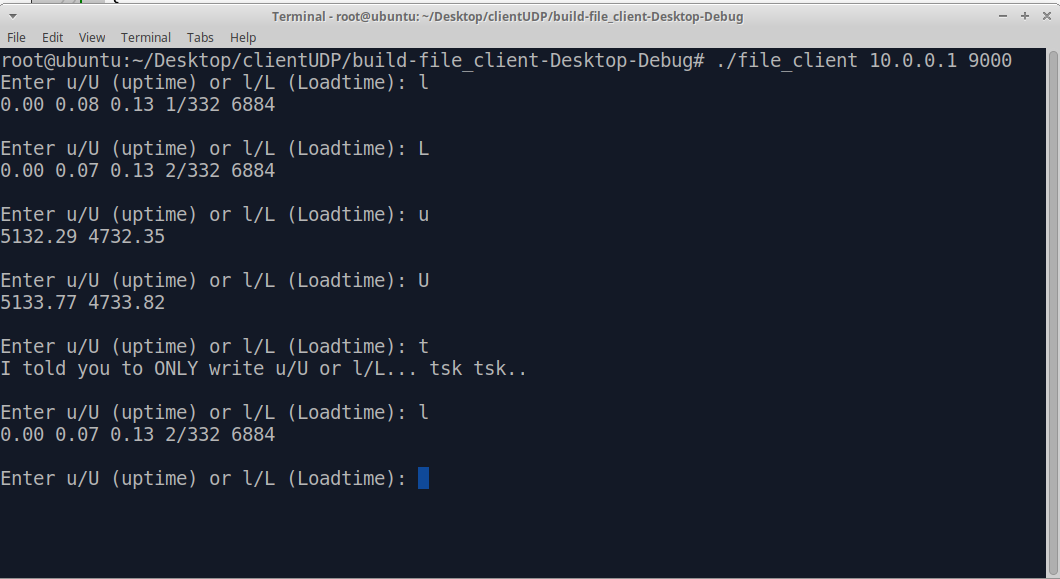
\includegraphics[width=0.9 \textwidth]{resultat_udp_client.png}
	\captionof{figure}{Skærmbillede taget af terminalen på klient-siden, hvor det ses at den modtager data fra serveren alt efter hvad brugerinputtet er.}
	\label{fig:resultat_udp_client}
\end{center}

\section{Server}
\begin{center}
	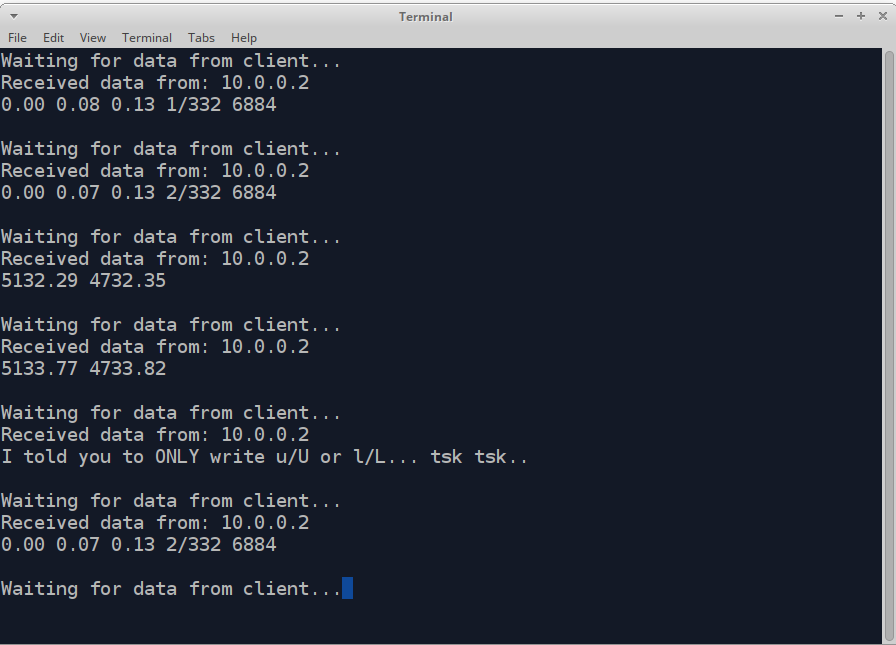
\includegraphics[width=0.9 \textwidth]{resultat_udp_server.png}
	\captionof{figure}{Skærmbillede taget af terminalen på server-siden, hvor det ses at den modtager data fra klienten, behandler det og sender data tilbage. Derfeter står den igen og venter på at modtage ny data.}
	\label{fig:resultat_udp_server}
\end{center}

\newpage


\end{document}